\documentclass[a4paper,11pt,onecolumn]{memoir}

\usepackage[utf8]{inputenc}
\usepackage[T1]{fontenc}
\usepackage[english]{babel}
% \usepackage[final]{microtype}

\usepackage{amsmath,amssymb,mathtools}

\usepackage[normalem]{ulem}

\usepackage{graphicx}

\usepackage{hyperref}
\hypersetup{
    pdfauthor={Thanh Dinh Ta}
}

\usepackage{subcaption}

\usepackage[backend=biber,style=alphabetic]{biblatex}
\usepackage{csquotes}
\addbibresource{inferix.bib}

% \setcounter{secnumdepth}{6}

\author{
    Inferix team
}
\title{Inferix's Proof of Rendering Algorithm}

\begin{document}

% \pagenumbering{arabic}

\frontmatter

\maketitle

\begin{abstract}
    This document presents the Active Noise Generation and Verification algorithm employed to verify image and video outputs of Inferix distributed graphics rendering service. This algorithm is the first effort introducing asymmetric watermarks into pre-rendering graphics scenes, it is different from classical watermarking method which can only work on media data.
\end{abstract}
\clearpage

\tableofcontents*
\clearpage

\mainmatter

\chapter{Introduction}
Inferix provides a decentralized graphics rendering service: remote people can submit Blender scenes then receive rendered images and videos, others can join the service to let their computing resources for hire. Since the graphic rendering processes are \sout{notoriously} intensively resources (GPU, RAM, disk storage, etc.) consuming and not everyone possessing these resources, Inferix regulates this exigence by in the one hand helping artists get their jobs done without equipping very high-end workstations. In the other hand, it allows individuals making profit from their unused high-performance computation resources.


\section[Rendering service]{Rendering service}
Inferix rendering services consists in a network of physically decentralized machines called \emph{nodes} which are of $3$ kinds: \emph{manager}, \emph{worker} and \emph{verifier}. The number of \emph{workers} is much larger than the number of \emph{managers} and \emph{verifiers}.

A rendering session is as follows: a user submits Blender scenes to a \emph{manager} directly using the Inferix plugin for Blender (or via some Web interface!?). The \emph{manager} creates a job corresponding to this graphics scene, queues this job into a pool then dispatches to \emph{workers} which do the rendering. The rendered images will be sent back from \emph{workers} to several \emph{verifiers} which check if the images are valid. The validity is notified to the \emph{manager} to accept or reject the rendered results: a job is considered valid only if all results of this job pass the verification, in this case the results will be sent back to users.

(...add a figure here describing the high-level architect of rendering service)

\section[Output verification]{Output verification}\label{sec:output_verification}
In the network, \emph{workers} are mostly workstations (beside Inferix's dedicated servers) joined by users which want to make profit from their unused computing resources. There is no control (except initial hardware requirements to join the network!?) over these machines, so the graphics rendering is proceeded without being controlled. In order to guarantee that the graphics scenes are correctly rendered, we propose a mechanism called \emph{Active Noise Generation and Verification} which is presented in detail in~\autoref{ch:scene_watermarking}.

(...add a concrete example about an attack)

\chapter{Scene watermarking}\label{ch:scene_watermarking}
Before being sent back to the users, the output images of \emph{workers} must be checked if they are actually the results of the corresponding submitted graphics scene. By architectural design, Inferix gains no control whatsoever on \emph{workers} (see~\ref{sec:output_verification}), the graphics rendering softwares installed on \emph{workers} always suffer from risks of being completely analyzed, reversed and maliciously modified. In the long run, one cannot make any assumption about the security on the \emph{worker}'s side, even worse \emph{workers} should be considered adversaries who exhaustively try to bypass any security enforcement applied on their side.
% , one cannot suppose any security on 
% the graphics rendering programs installed on workers are secured.

A public-key cryptography approach is using a scheme of \emph{fully homomorphic encryption} (FHE)~\cite{Gentry2009}. The graphics scene is encrypted first by a private key before sending to \emph{workers}. Given the corresponding public key, the homomorphic encryption software performs the graphics rendering on the encrypted scene without needing to decrypt it. Finally, the encrypted rendered results are returned and decrypted at the user's side using the private key. The advantage of FHE is that the \emph{workers}, even can modify the FHE softwares on their side, cannot interfere the FHE graphics rendering processes without being detected. Unfortunately, this approach is impractical since all state-of-the-art implementations will make the performance of the homomorphic encryption graphics rendering become unacceptable~\cite{9910347}.

To handle this problem, we use a watermarking~\cite{Cox1997,Cox1999} method called \emph{Active Noise Generation and Verification} (ANGV) which is a simpler variant of \emph{proof of ownership}~\cite{Craver1997} schemes. \emph{First}, the detector can always judge that the rendered digital content is the result of a valid rendering process whose input is the submitted graphics scene. \emph{Second}, though ANGV needs to modify the initial submitted scene, as a sequence the rendered output will be distorted also, the distortion is regulated to below the human perception capability, so there is no quality degradation. \emph{Third}, the embedded watermark is robust under rendering enhancements (e.g. anti-aliasing) and post-processing operations. \emph{Finally}, there is no need to use a special rendering software on \emph{workers} as in the case of FHE, the performance of graphics rendering will be not affected.
% verification will be proceeded on \emph{verifiers}

% the verification is proceeded on \emph{verifiers}

\section[Active noise generation and verification]{Active noise generation and verification}
% As discussed above (see also~\ref{sec:output_verification}), to check the validity of the rendered images output from \emph{workers}, special watermarks will be embedded into these images.
% It is important to note that we cannot insert watermarks into the images as in the traditional digital watermarking methods~\cite{Cox2008} since the images are output of \emph{workers}, they are not under our control.
% Since images are output of \emph{workers} which are not under control, watermarks cannot be embedded directly into 
The user submits some Blender work to the \emph{manager}, this work consists of several graphics scenes. Each scene contains information about graphical objects, the camera, light sources and materials~\cite{Blender}. The photorealistic rendering is a sophisticated computation process that calculate light properties at surfaces of all visible objects, results in 3D rendered images of the scene~\cite{Hughes2014}.

To check whether an image output from a \emph{worker} is actually the result of a valid graphics rendering process whose input is a given scene, invisible watermarks~\cite{Craver1997} will be embedded into the rendered images. A \emph{verifier} which knows the watermarks  It might be worth noting that, different from the context of traditional digital watermarking schemes~\cite{Cox2008}, these images are not under our control, they are instead output of \emph{workers}. Hence, it is not possible to embed directly watermarks into images, our approach is to embed watermarks into the graphics scene submitted by users before sending it to \emph{workers}.
% the initial digital content in this context is now the output of the malicious side, so freely susceptible to malicious intervention.

\subsection[Hight level description]{High level description}
The \emph{Active Noise Generation and Verification} (ANGV) consists of two main procedures as described below.

\paragraph[Watermark insertion]{Watermark insertion}
In practice, a graphics scene may have multiple frames and each worker may render only a subset of these frames. For the simplification purpose, we assume in this section that a scene has only one frame, so the output rendered image is determined uniquely by the scene.

Let $\mathcal{R}$ and $S$ denote respectively the rendering function and the scene, the rendered image $I$ without watermark will be:
\begin{equation*}
    I = \mathcal{R} \left( S \right)
\end{equation*}
It is important to note that $I$ is actually never computed (neither by the \emph{manager} in the watermark insertion procedure nor by \emph{workers} in rendering processes), the equation above represents only an equality. Similar with traditional schemes~\cite{Cox1999,Cox1997,Craver1997}, a watermark $W$ is a sequence of atomic watermarks:
\begin{equation*}
    W = \left\{ w_1,\dots,w_n \right\}
\end{equation*}
where $w_i$ is chosen from some probability distribution and $w_i$ may also depend on $S$ (see~\autoref{par:robustness}). Using $W$ and $S$, we next generate a representative key:
\begin{equation*}
    K_{\mathtt{repr}} \left(W,S\right) = \left\{ k_1,\dots,k_n \right\}
\end{equation*}
that will be used later for the watermark verification procedure. We do not insert $W$ into the image $I$ but into the scene $S$ using an encoding function $\mathcal{E}$, to create a watermarked scene:
\begin{equation*}
    \hat{S} = \mathcal{E} \left(S, W\right)
\end{equation*}
Finally $\hat{S}$ is sent to \emph{workers} for rendering, that results in a watermarked image:
\begin{equation*}
    \hat{S} = \mathcal{R} \thinspace (\hat{S})
\end{equation*}

\paragraph[Watermark verification]{Watermark verification}
Given an image $\hat{I}$ and a representative key $K_{\mathtt{repr}}$, we first try to recover a watermark $\hat{W}$ from $\hat{I}$ using a decoding function $\mathcal{D}$:
\begin{equation*}
    \hat{W} = \mathcal{D} \thinspace (\hat{I}, K_{\mathtt{repr}})
\end{equation*}
Next $\hat{W}$ is compared against $W$, if the difference is above some threshold $T$
\begin{equation*}
    \lVert \hat{W} - W \rVert \geq T
\end{equation*}
then $\hat{I}$ will be accepted otherwise rejected.

\paragraph[Rendering result]{Rendering result}
In case of being accepted, the rendered image sent back to users is $\hat{I} = \mathcal{R}\thinspace(\hat{S})$ but not $I = \mathcal{R}\left(S\right)$. The encoding function $\mathcal{E}$ and the watermark $W$ are designed so that the distortion of $\hat{I}$ against $I$ is under human perception capability, then $\hat{I}$ can be authentically used as a result of the graphics rendering.

\paragraph[Performance]{Performance}
The functions $\mathcal{E}$ and $\mathcal{D}$ are designed so that their computation resource consumption is negligible in comparison with the graphics rendering function $\mathcal{R}$; and the watermark verification does not require $I$, only $\hat{I}$ is rendered. That means the only overhead caused by ANGV is by $\mathcal{E}$ and $\mathcal{D}$, hence there is no significant effect on the performance of the graphics rendering.
% (there is no need to render this image for comparing with $I'$)
 

\subsection[Implementation]{Implementation}
In this section, we present in detail the current Inferix's implementation of watermark insertion and verification.

% \subsubsection[Insertion]{Insertion}

\paragraph[Structure of watermark]{Structure of watermark}\label{par:structure_of_watermark}
As described above, a watermark $W$ consists of a sequence of $n$ atomic watermarks, each watermark $w_i$ is a rectangle image of special pattern (see~\autoref{fig:atomic_patterns}) of noise chosen from a normal distribution $w_i \sim \mathcal{N}(0, \sigma_i^2)$.
\begin{figure}[h]
    \centering
    \begin{subfigure}[b]{0.25\textwidth}
        
\includegraphics[width=\textwidth]{w_inferix_0.png}
    \end{subfigure}
    \qquad
    \begin{subfigure}[b]{0.25\textwidth}
        
\includegraphics[width=\textwidth]{w_inferix_1.png}
    \end{subfigure}
    \caption[Some atomic watermark patterns]{Some atomic watermark patterns}
    \label{fig:atomic_patterns}
\end{figure}
% \begin{figure}[h]
%     \centering
%     
\includegraphics[scale=0.2]{w_inferix.png}
%     \caption{An atomic watermark}
%     \label{fig:atomic_watermark}
% \end{figure}
The number $n$ is one of the factors decides the robustness of watermark, the higher this number the lower the false positive of watermark verification. Experimentally, $W$ contains about $8$ to $10$ atomic watermarks.

\paragraph[Watermark insertion]{Watermark insertion}
Given some graphics scene $S$, we embed the watermark $W$ into $S$ by wrapping each atomic watermark as a graphics objects, then insert these objects into $S$ so that they contribute to the result rendered image (i.e. they distort this image).

By the nature of the graphics rendering, an object in the scene will not be visible if there is no light scattered from the surface of the object to the camera. This may be caused by several reasons: the object is not located in the frustum of the camera, is hidden by some other objects, or the material of the object is transparent, etc. The watermark insertion must satisfy first several constraints:
\begin{itemize}
    \item there are no collisions between watermark objects,
    \item all watermark objects are located completely in the camera frustum,
    \item no watermark object is hidden by another object (including both watermark objects and existing objects of the scene).
\end{itemize}

\paragraph[Representative key generation]{Representative key generation}
An atomic watermark $w_i$ contributes to the image $\hat{I}$ as a rectangular region at the location $k_i$ (for that, the rotation vector of the graphics object $w_i$ is kept to be equal with the one of the camera in $S$). The location $k_i$ on $\hat{I}$ can be precisely calculated without rendering:
\begin{equation*}
    k_i = \left(x^{\mathtt{ul}}_i, y^{\mathtt{ul}}_{i},x^{\mathtt{lr}}_i, y^{\mathtt{lr}}_{i}\right)
\end{equation*}
where $\left(x^{\mathtt{ul}}_i, y^{\mathtt{ul}}_{i}\right)$ (resp. $x^{\mathtt{lr}}_i, y^{\mathtt{lr}}_{i}$) are the upper left (resp. lower right) coordinates of the region. So the insertion of $W$ into $S$ generates a key
\begin{equation*}
    K_{\mathtt{repr}} = \left\{k_1,\dots,k_n \right\}
\end{equation*}

\paragraph[Other constraints]{Other constraints}
It might be worth noting that $k_i$ represents the distortion caused by the atomic watermark $w_i$ to the rendered image, normally $k_i$ is much smaller than the original size of $w_i$. On the one hand $k_i$ must not be negligible otherwise the watermark verification is not possible. On the other hand, $k_i$ must be kept under the human perception capability. Experimentally we keep a trade-off:
\begin{align}\label{eq:side_constraint}
\begin{split}
    2 \leq x^{\mathtt{lr}}_{i} - x^{\mathtt{ul}}_{i} \leq 3 \\
    2 \leq y^{\mathtt{lr}}_{i} - y^{\mathtt{ul}}_{i} \leq 3
\end{split}
\end{align}
for all $1 \leq i \leq n$ (see~\autoref{fig:coca_cola} and~\autoref{fig:tea_mug}).
\begin{figure}[ht]
    \centering
    \makebox[\textwidth][c]{%
    \begin{subfigure}[t]{0.4\textwidth}
        \centering
        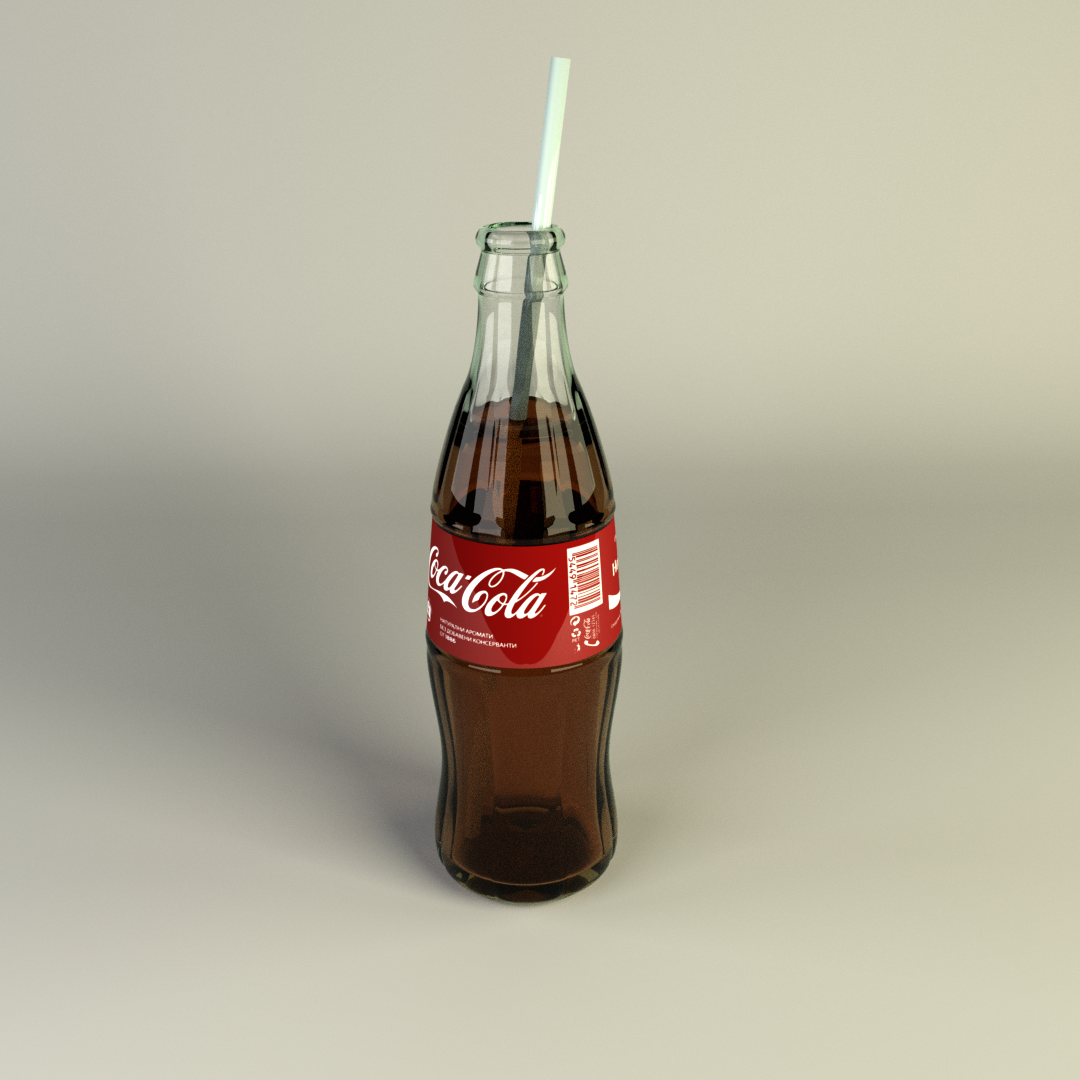
\includegraphics[width=\textwidth]{coca_cola.png}
        \label{subfig:coca_cola}
        \caption{Original}
    \end{subfigure}
    % \quad
    \begin{subfigure}[t]{0.4\textwidth}
        \centering
        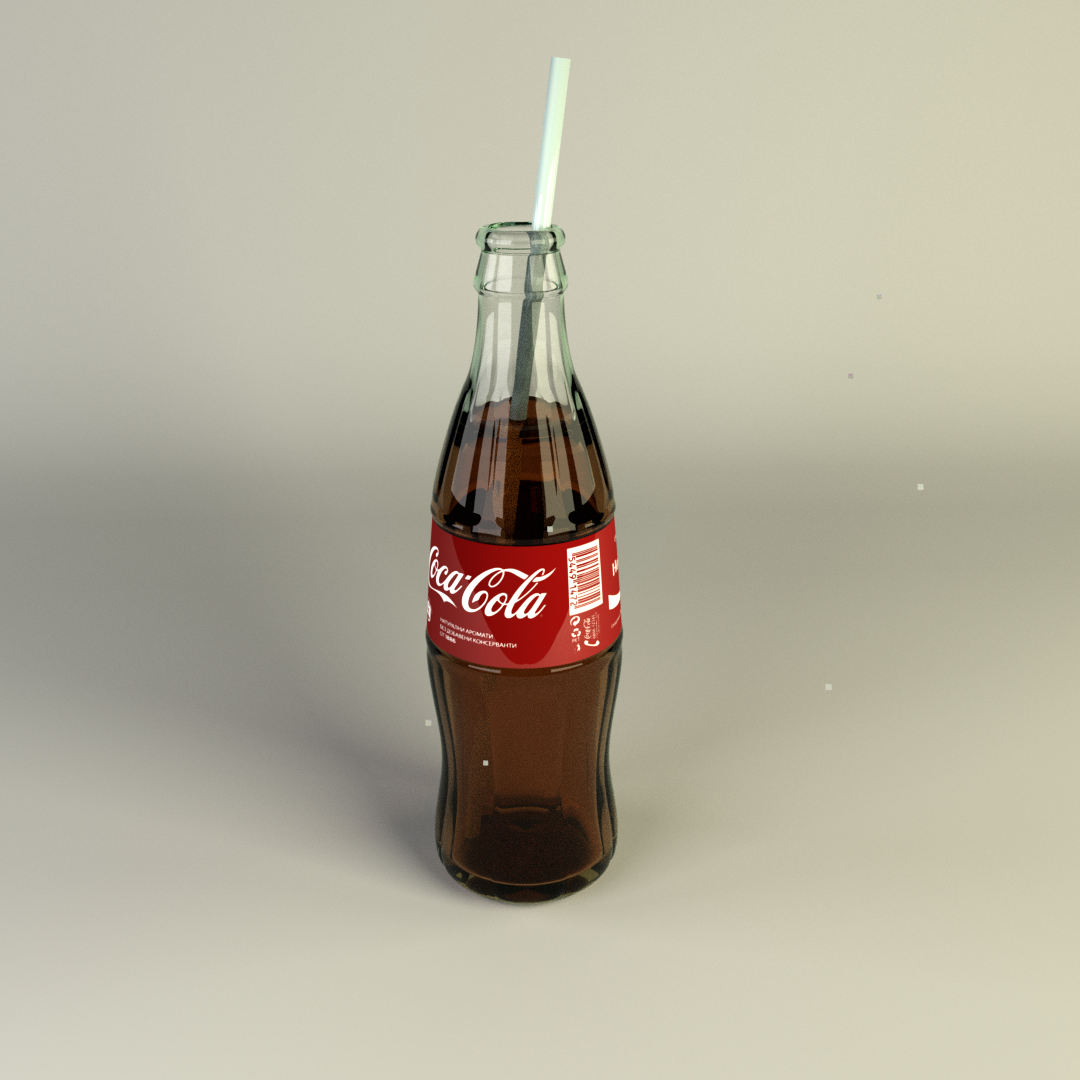
\includegraphics[width=\textwidth]{coca_cola_wm_ko.png}
        \label{subfig:coca_cola_wm_ko}
        \caption{Watermarked with atomic watermark size $= 5$}
    \end{subfigure}
    % \vfill
    % \qquad
    \begin{subfigure}[t]{0.4\textwidth}
        \centering
        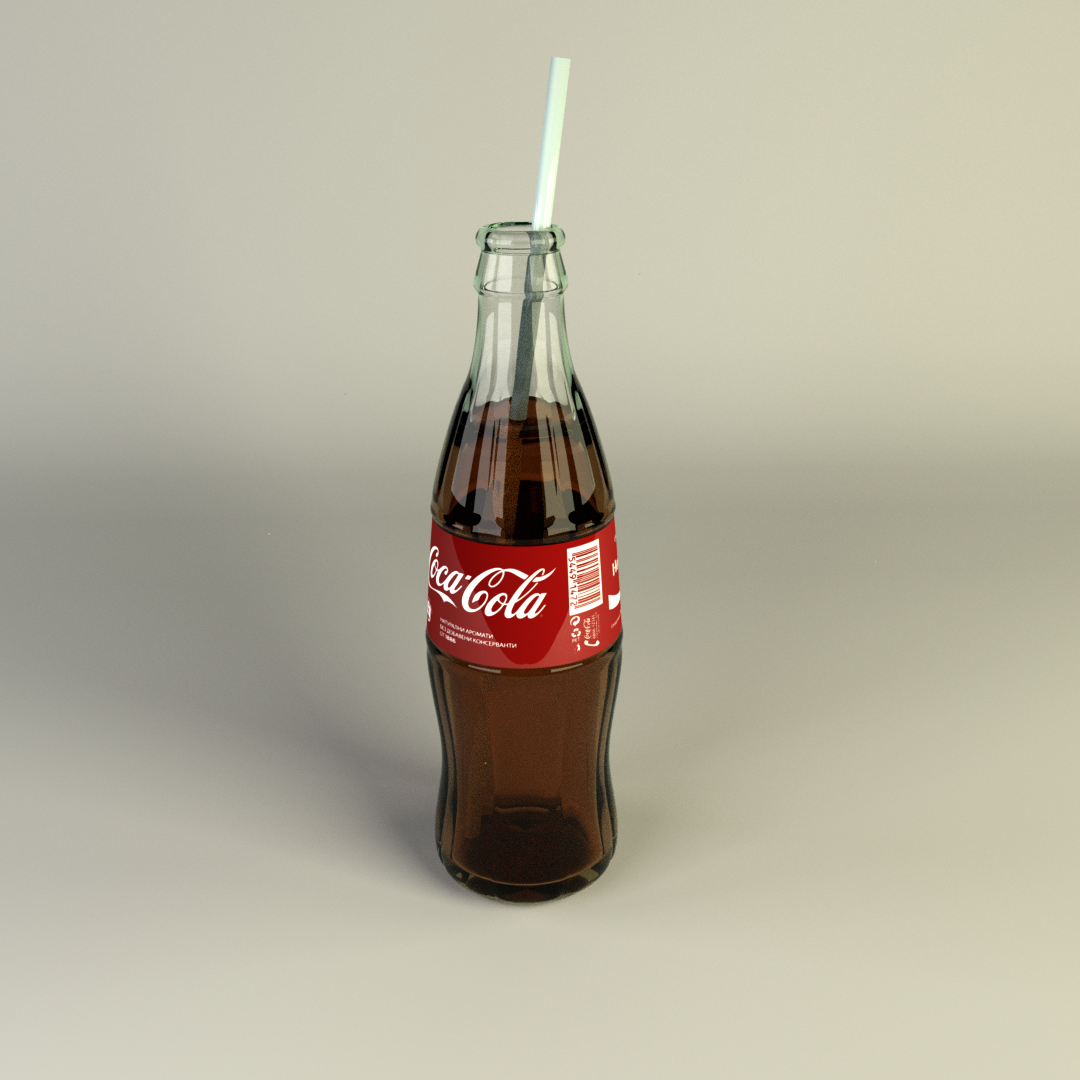
\includegraphics[width=\textwidth]{coca_cola_wm_ok.png}
        \label{subfig:coca_cola_wm_ok}
        \caption{Atomic watermark size $= 2$}
    \end{subfigure}}
    \caption[Scene watermarked with different sizes of atomic watermarks]{Scene watermarked with different size of atomic watermarks: the distortion is observable when the width and the height of an atomic watermark are about $5$, but unobservable when these lengths are $2$.}
    \label{fig:coca_cola}
\end{figure}

\begin{figure}[ht]
    \centering
    \makebox[\textwidth][c]{%
    \begin{subfigure}[t]{0.4\textwidth}
        \centering
        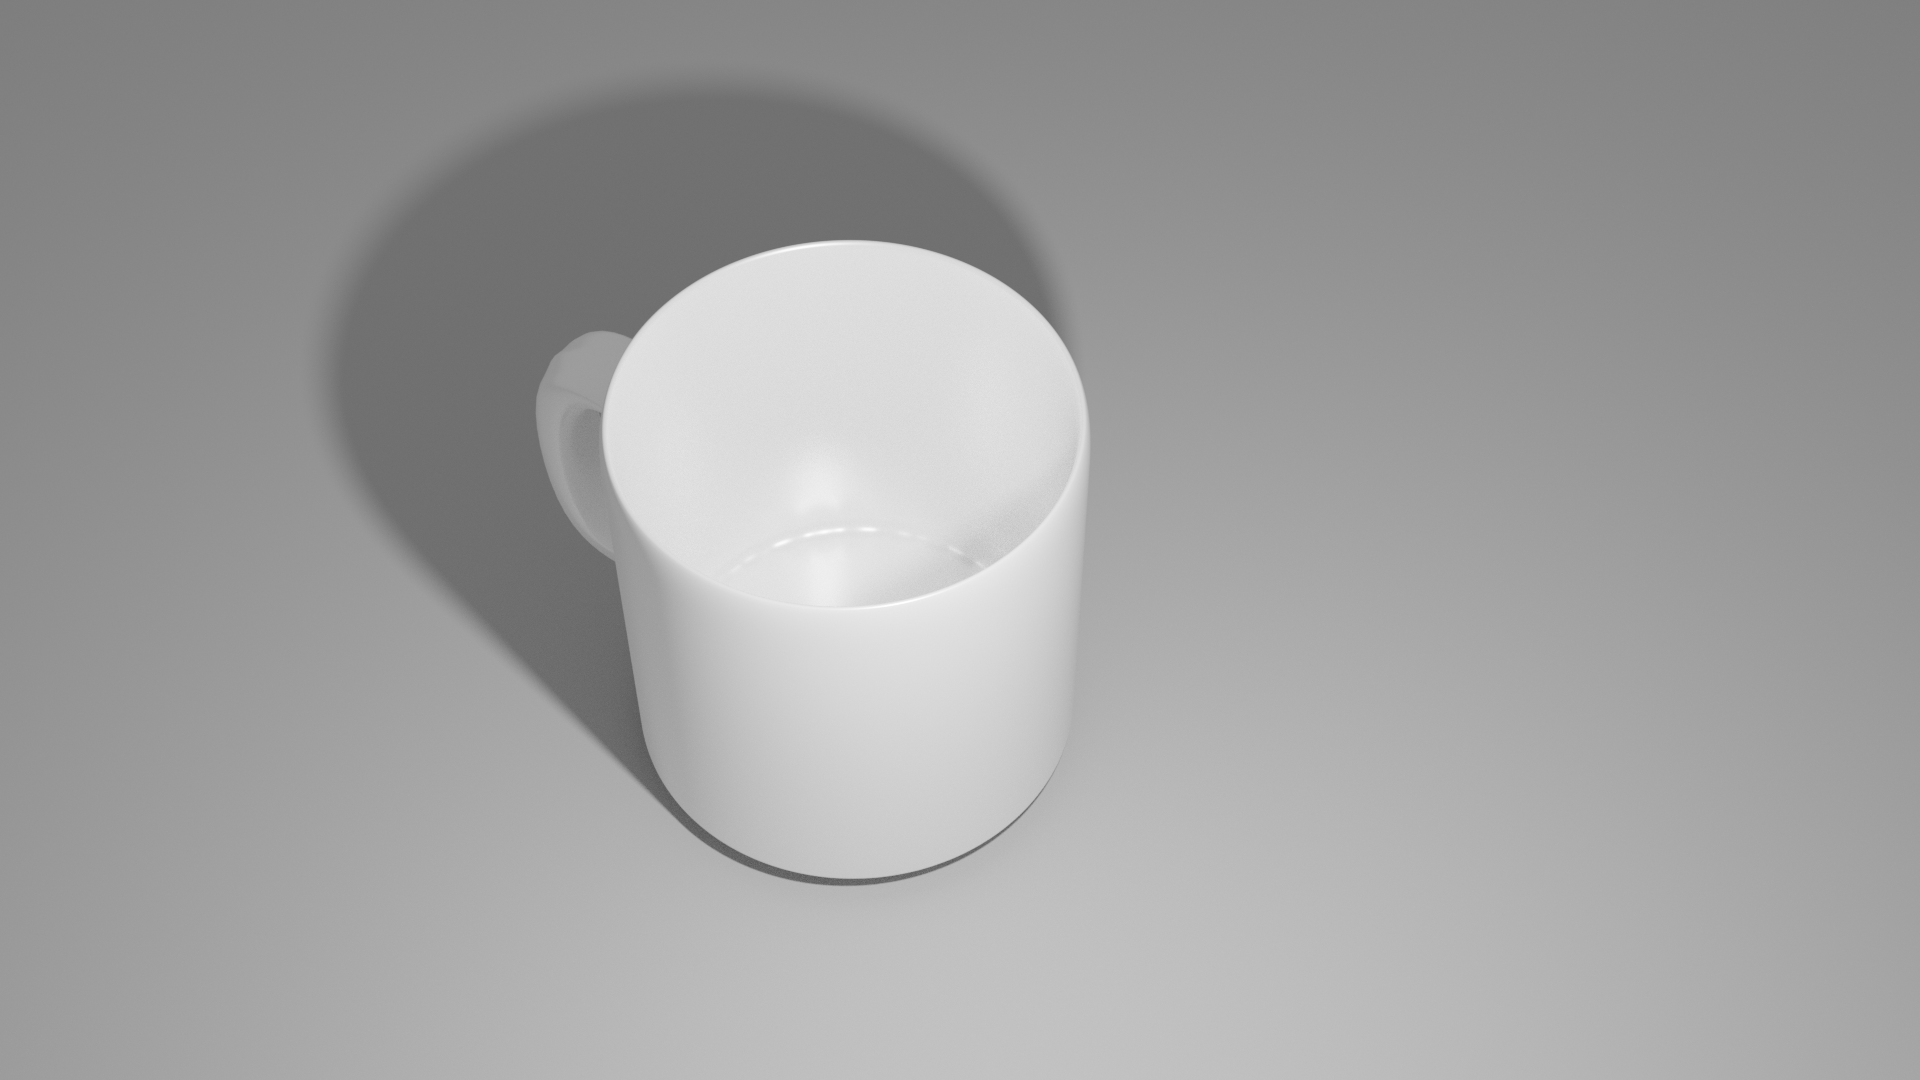
\includegraphics[width=\textwidth]{tea_mug.png}
        \label{subfig:tea_mug}
        \caption{Original}
    \end{subfigure}
    \begin{subfigure}[t]{0.4\textwidth}
        \centering
        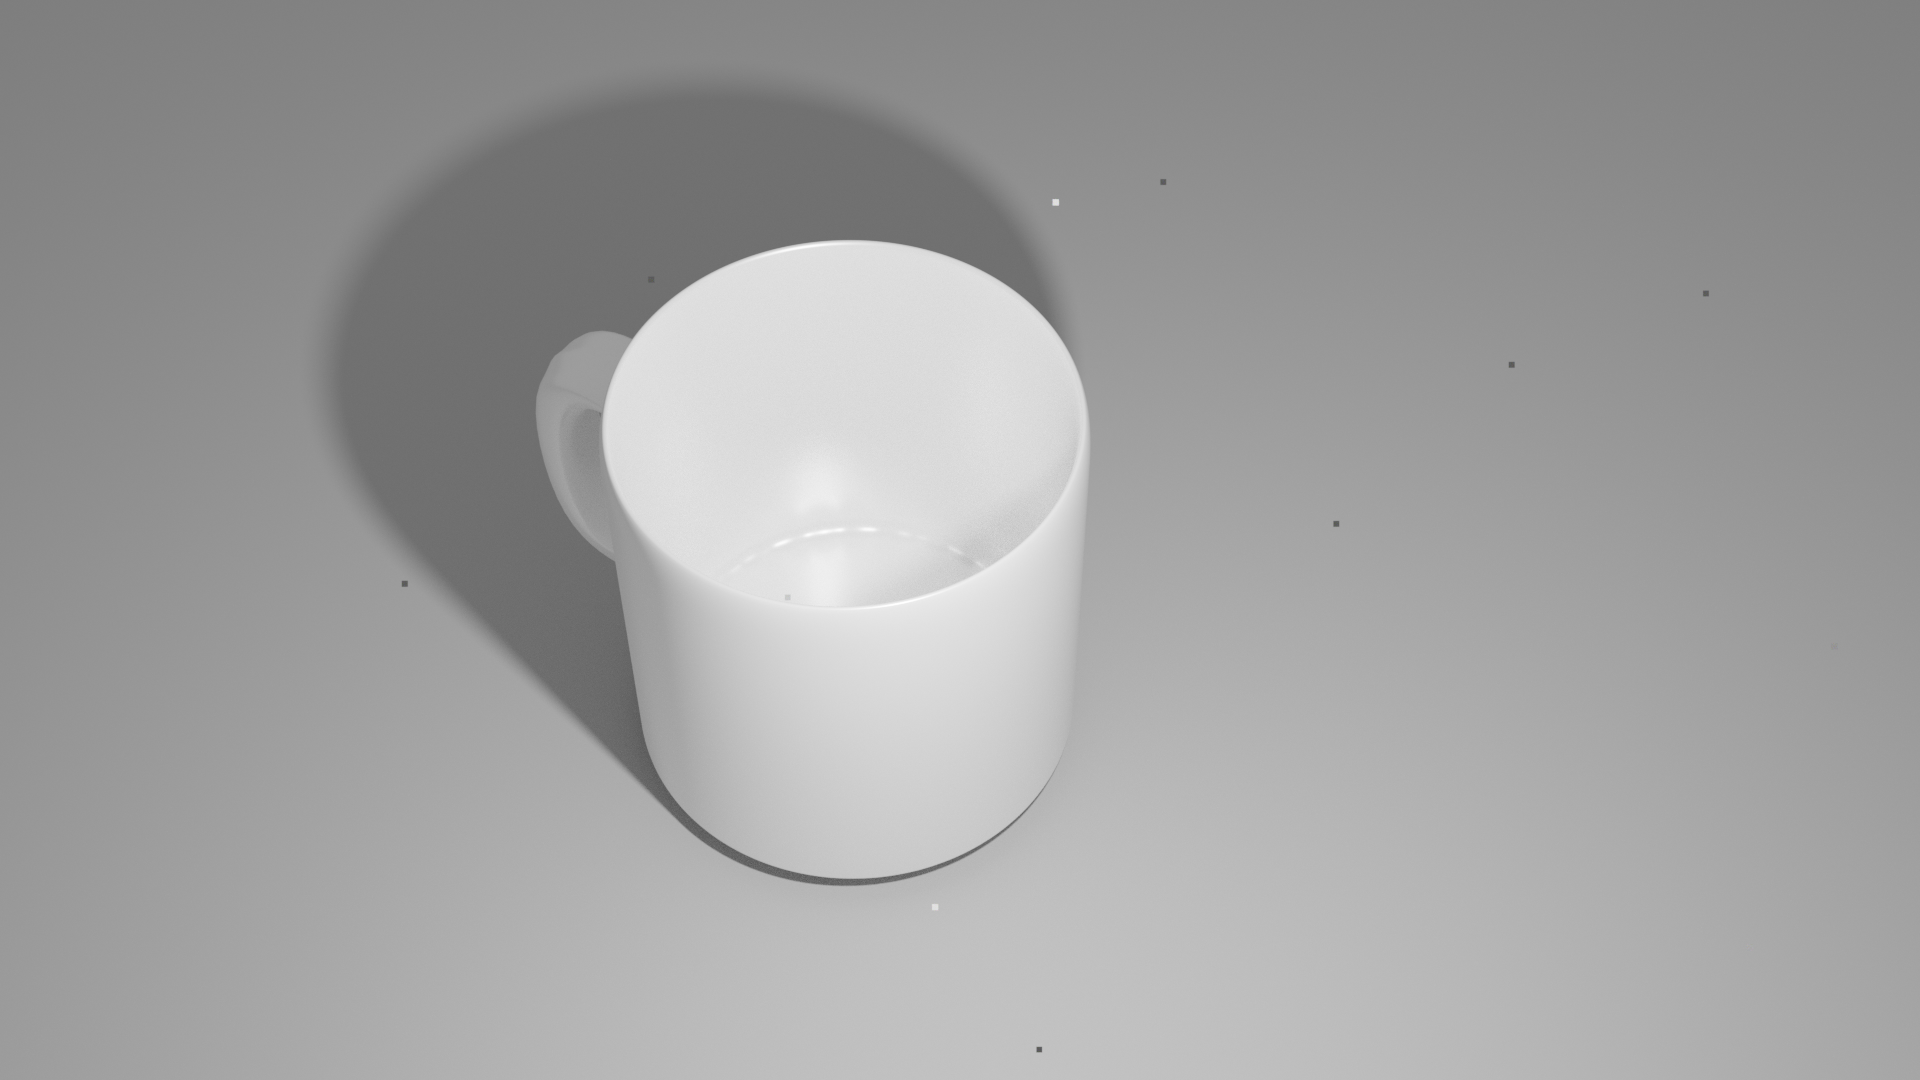
\includegraphics[width=\textwidth]{tea_mug_wm_ko.png}
        \label{subfig:tea_mug_wm_ko}
        \caption{Atomic watermark size $= 7$}
    \end{subfigure}
    \begin{subfigure}[t]{0.4\textwidth}
        \centering
        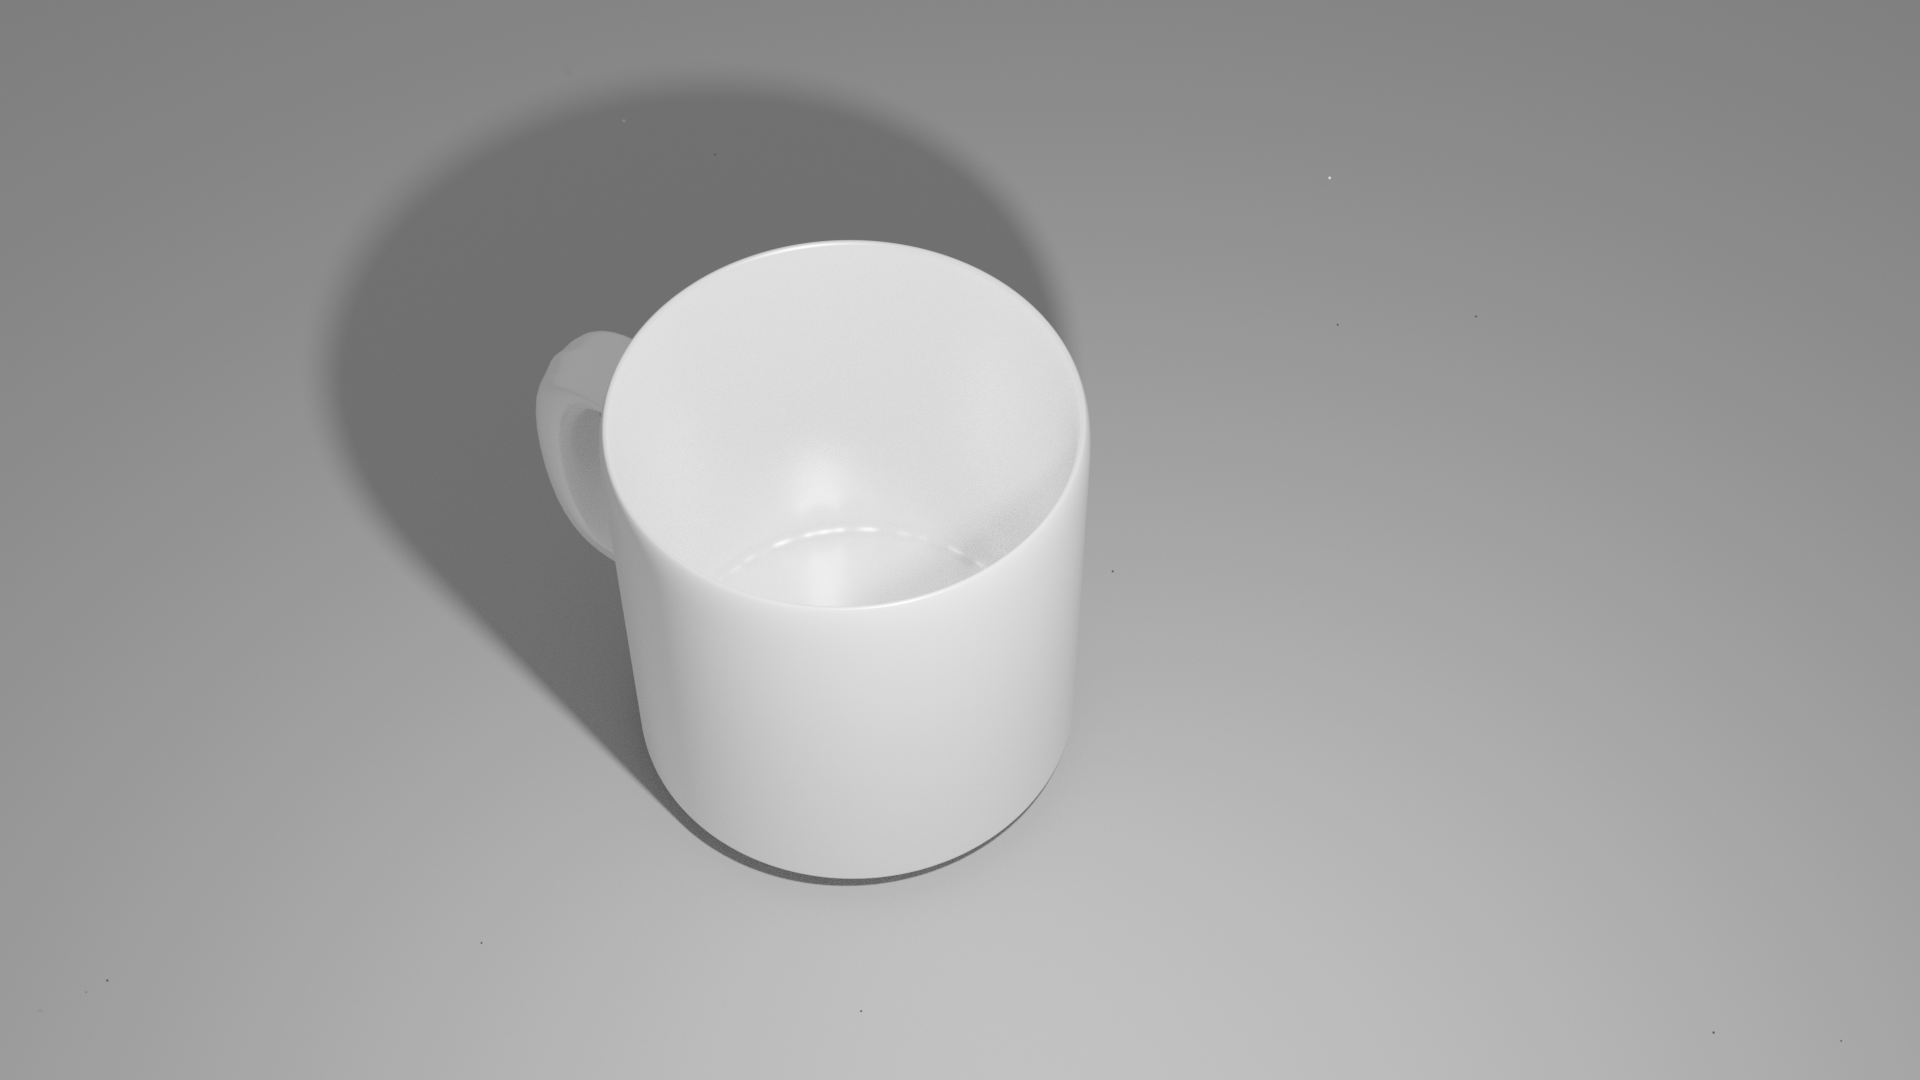
\includegraphics[width=\textwidth]{tea_mug_wm_ok.png}
        \label{subfig:tea_mug_wm_ok}
        \caption{Atomic watermark size $= 3$}
    \end{subfigure}}
    \caption[Scene watermarked with different sizes of atomic watermarks]{Another scene watermarked with different sizes of atomic watermarks}
    \label{fig:tea_mug}
\end{figure}

\paragraph[Watermark verification]{Watermark verification}
The verification procedure needs only the representative key $K_\mathtt{repr}$ and the rendered image $\hat{I}$. It is not always possible to restore the atomic watermark $w_i \in W$ since most information of $w_i$ is lost after the graphics rendering process (note that $k_i$ is much smaller than the size of $w_i$). However, it is neither necessary to restore $w_i$, instead to verify the existence of $W$, checking the existence of $w_i$ on the image region determined by $k_i$ on $\hat{I}$ for $1 \leq i \leq n$ is sufficient.

For each region of coordinates $k_i = \left(x^{\mathtt{ul}}_i, y^{\mathtt{ul}}_{i},x^{\mathtt{lr}}_i, y^{\mathtt{lr}}_{i}\right)$, we pick a bound region of coordinates:
\begin{equation*}
    b_i =  \left(x^{\mathtt{ul}}_i - \delta^{x}_{i}, y^{\mathtt{ul}}_{i} - \delta^{y}_i ,x^{\mathtt{lr}}_i + \delta^{x}_{i}, y^{\mathtt{lr}}_{i} + \delta^{y}_{i}\right)
\end{equation*}
where $\delta^{x}_{i}$ and $\delta^{y}_{i}$ are the width and the height of $k_i$ (see~\autoref{subfig:coca_cola_pickup}):
\begin{equation*}
    \delta^{x}_{i} = x^{\mathtt{lr}}_i - x^{\mathtt{ul}}_i \qquad \delta^{y}_{i} = y^{\mathtt{lr}}_i - y^{\mathtt{ul}}_i \\
\end{equation*}
To check the contribution of the atomic watermark at the region of coordinates $k_i$, we apply an edge detection filter (see~\autoref{subfig:coca_cola_pickup_filtered}) on the bound region, then compare the mean $m_b$ of the bound region against the mean $m_k$ of the atomic watermark located inside. Experimentally, we will check if
\begin{equation}\label{eq:edge_difference}
    m_k - m_b \geq 5
\end{equation}
to validate the existence of the atomic watermark. This check is proceeded for all $n$ atomic watermarks, if all of them are validated then the rendered image $\hat{I}$ is accepted otherwise rejected.
\begin{figure}[ht]
    \centering
    \begin{subfigure}[t]{0.45\textwidth}
        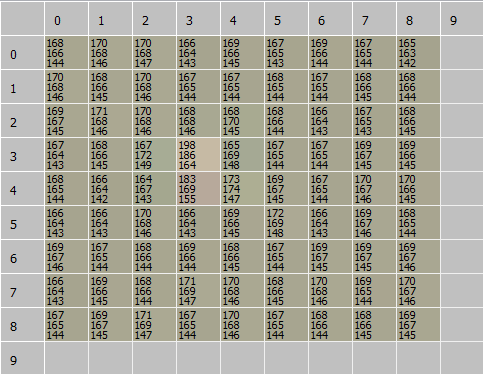
\includegraphics[width=\textwidth]{coca_cola_bound.png}
        \caption{Pickup bound region of size $9\times9$ pixels, the atomic watermark region of size $3\times3$ located at the center of the bound (numbers on each pixel are RGB color values)}
        \label{subfig:coca_cola_pickup}
    \end{subfigure}
    \qquad
    \begin{subfigure}[t]{0.45\textwidth}
        
\includegraphics[width=\textwidth]{coca_cola_laplace.png}
        \caption{Pickup bound region after an edge detection filter}
        \label{subfig:coca_cola_pickup_filtered}
    \end{subfigure}
    \caption{Watermark verification}
    \label{fig:coca_cola_bound}
\end{figure}

\paragraph[Robustness]{Robustness}\label{par:robustness}
We now discuss several details about the contribution of the watermark on the rendered image. There are two related constraints:
\begin{itemize}
    \item the side trade-off in~\autoref{eq:side_constraint} is used to keep the rendering distortion under the human perception capability, and
    \item the mean difference in~\autoref{eq:edge_difference} is used to validate the existence of an atomic watermark
\end{itemize}
which are unfortunately disproportional: if the side is too small

\subsection[Performance]{Performance}

\section[Threat analysis]{Threat analysis}


% \chapter{Asymmetric watermarking}
% This should be the hardest chapter~\dots

\backmatter

\printbibliography

\end{document}